% This file was created with tikzplotlib v0.10.1.
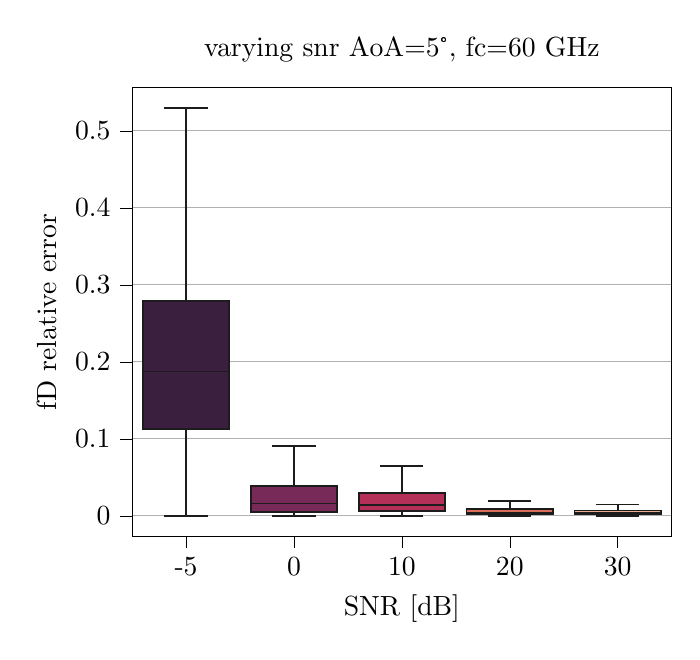
\begin{tikzpicture}

\definecolor{black28}{RGB}{28,28,28}
\definecolor{brown1814888}{RGB}{181,48,88}
\definecolor{burlywood231175145}{RGB}{231,175,145}
\definecolor{darkgray176}{RGB}{176,176,176}
\definecolor{darkslategray583162}{RGB}{58,31,62}
\definecolor{indianred21811088}{RGB}{218,110,88}
\definecolor{purple1194288}{RGB}{119,42,88}

\begin{axis}[
tick align=outside,
tick pos=left,
title={varying snr AoA=5°, fc=60 GHz},
x grid style={darkgray176},
xlabel={SNR [dB]},
xmin=-0.5, xmax=4.5,
xtick style={color=black},
xtick={0,1,2,3,4},
xticklabels={-5,0,10,20,30},
y grid style={darkgray176},
ylabel={fD relative error},
ymajorgrids,
ymin=-0.0264670081718795, ymax=0.555817057296555,
ytick style={color=black}
]
\path [draw=black28, fill=darkslategray583162, semithick]
(axis cs:-0.4,0.112752411423856)
--(axis cs:0.4,0.112752411423856)
--(axis cs:0.4,0.279421575228086)
--(axis cs:-0.4,0.279421575228086)
--(axis cs:-0.4,0.112752411423856)
--cycle;
\path [draw=black28, fill=purple1194288, semithick]
(axis cs:0.6,0.00483968162025414)
--(axis cs:1.4,0.00483968162025414)
--(axis cs:1.4,0.0390423175890101)
--(axis cs:0.6,0.0390423175890101)
--(axis cs:0.6,0.00483968162025414)
--cycle;
\path [draw=black28, fill=brown1814888, semithick]
(axis cs:1.6,0.00623714968679289)
--(axis cs:2.4,0.00623714968679289)
--(axis cs:2.4,0.0297488868954462)
--(axis cs:1.6,0.0297488868954462)
--(axis cs:1.6,0.00623714968679289)
--cycle;
\path [draw=black28, fill=indianred21811088, semithick]
(axis cs:2.6,0.00165840950639557)
--(axis cs:3.4,0.00165840950639557)
--(axis cs:3.4,0.00862670364523936)
--(axis cs:2.6,0.00862670364523936)
--(axis cs:2.6,0.00165840950639557)
--cycle;
\path [draw=black28, fill=burlywood231175145, semithick]
(axis cs:3.6,0.00152428100463443)
--(axis cs:4.4,0.00152428100463443)
--(axis cs:4.4,0.0067780315749917)
--(axis cs:3.6,0.0067780315749917)
--(axis cs:3.6,0.00152428100463443)
--cycle;
\addplot [semithick, black28]
table {%
0 0.112752411423856
0 5.7990351072108e-05
};
\addplot [semithick, black28]
table {%
0 0.279421575228086
0 0.529349599775262
};
\addplot [semithick, black28]
table {%
-0.2 5.7990351072108e-05
0.2 5.7990351072108e-05
};
\addplot [semithick, black28]
table {%
-0.2 0.529349599775262
0.2 0.529349599775262
};
\addplot [semithick, black28]
table {%
1 0.00483968162025414
1 1.01708506732851e-06
};
\addplot [semithick, black28]
table {%
1 0.0390423175890101
1 0.0902886490668191
};
\addplot [semithick, black28]
table {%
0.8 1.01708506732851e-06
1.2 1.01708506732851e-06
};
\addplot [semithick, black28]
table {%
0.8 0.0902886490668191
1.2 0.0902886490668191
};
\addplot [semithick, black28]
table {%
2 0.00623714968679289
2 1.24488261860948e-06
};
\addplot [semithick, black28]
table {%
2 0.0297488868954462
2 0.0650121055563858
};
\addplot [semithick, black28]
table {%
1.8 1.24488261860948e-06
2.2 1.24488261860948e-06
};
\addplot [semithick, black28]
table {%
1.8 0.0650121055563858
2.2 0.0650121055563858
};
\addplot [semithick, black28]
table {%
3 0.00165840950639557
3 4.49349412955034e-07
};
\addplot [semithick, black28]
table {%
3 0.00862670364523936
3 0.0190738797471753
};
\addplot [semithick, black28]
table {%
2.8 4.49349412955034e-07
3.2 4.49349412955034e-07
};
\addplot [semithick, black28]
table {%
2.8 0.0190738797471753
3.2 0.0190738797471753
};
\addplot [semithick, black28]
table {%
4 0.00152428100463443
4 2.74806254249185e-06
};
\addplot [semithick, black28]
table {%
4 0.0067780315749917
4 0.0146411382358419
};
\addplot [semithick, black28]
table {%
3.8 2.74806254249185e-06
4.2 2.74806254249185e-06
};
\addplot [semithick, black28]
table {%
3.8 0.0146411382358419
4.2 0.0146411382358419
};
\addplot [semithick, black28]
table {%
-0.4 0.187614354360628
0.4 0.187614354360628
};
\addplot [semithick, black28]
table {%
0.6 0.0160903551636828
1.4 0.0160903551636828
};
\addplot [semithick, black28]
table {%
1.6 0.0140988324219269
2.4 0.0140988324219269
};
\addplot [semithick, black28]
table {%
2.6 0.00401879930179878
3.4 0.00401879930179878
};
\addplot [semithick, black28]
table {%
3.6 0.00371633159647347
4.4 0.00371633159647347
};
\end{axis}

\end{tikzpicture}
